\chapter{Protezione Dati Sensibili}

\section{Introduzione}
Molti DB contengono \textbf{dati sensibili}, che si definiscono come quei dati che \underline{non dovrebbero essere resi pubblici}.
La identificazione dei dati sensibili dipende molto dal \textbf{DB} e dalla sua specifica \underline{applicazione}.
I due casi estremi di questa categorizzazione sono : 
\begin{itemize}
\item \underline{Nessun} dato sensibile (ad es. il catalogo di una biblioteca)
\item \underline{Tutti} dati sensibili (ad es. un database della difesa militare)
\end{itemize}
Questi sono, inoltre, i casi più semplici da gestire, in quanto si \underline{garantisce} accesso a tutto il DB o si \underline{nega} accesso a tutto il DB.
In generale si ha che solo \textbf{alcuni dati sono sensibili} e che, inoltre, ognuno presenta un \textbf{diverso livello di sensibilità} necessario da applicare.

\begin{figure}[htbp]
	\centering
	{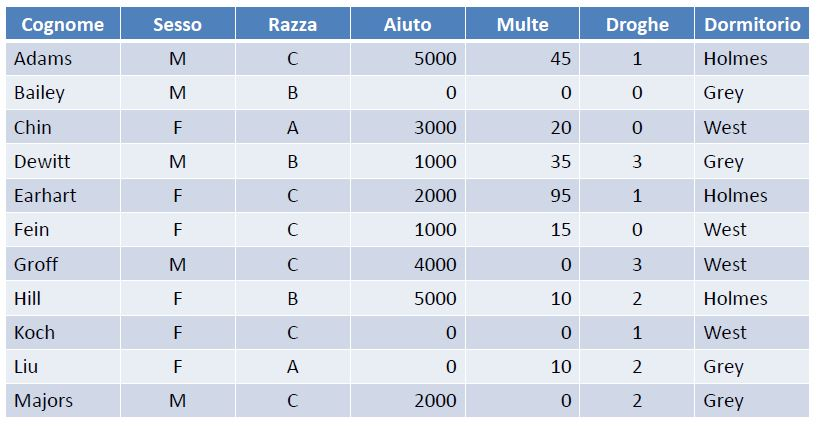
\includegraphics[height=15cm, width=12cm, keepaspectratio]{Immagini/Capitolo10/prot_dati_01.jpg}}
	\caption{Esempio di una tabella di un DB \label{fig:tabella_db}}
	
\end{figure}

Nella tabella di fig: \ref{fig:tabella_db} i Campi Non Sensibili risultano essere Nome e Dormitorio, quelli Sensibili sono Aiuto, Multe e Droghe mente quelli Parzialmente Sensibili sono Sesso e Razza.
I dati possono essere sensibili secondo i seguenti parametri:
\begin{itemize}

	\item \textbf{Sensibili per Contenuto}, in cui è il valore dell'attributo ad essere sensibile.
	\item \textbf{Sensibili per Provenienza}, in questo caso è la fonte dei dati a necessitare riservatezza.
	\item \textbf{Dichiarati Sensibili}, è lo stesso Amministratore del Sistema a dichiarare che i dati sono sensibili.
	
\end{itemize}

Le parti sensibili di un dato possono essere un \textbf{attributo o record}, un intero record o solo un certo attributo possono risultare sensibili; le parti sensibili lo possono essere sempre o \textbf{diventare sensibili in funzione alla divulgazione di altri dati}, ad esempio la longitudine di un sito segreto non è sensibile finché non è fornito insieme alla latitudine.

Il come non divulgare dati sensibili può non essere semplice, infatti si possono ottenere dati sensibili anche se i dati in sè non vengono mostrati, perciò anche alcune delle caratteristiche dei dati devono essere considerate sensibili.

\begin{figure}[htbp]

	\centering
		{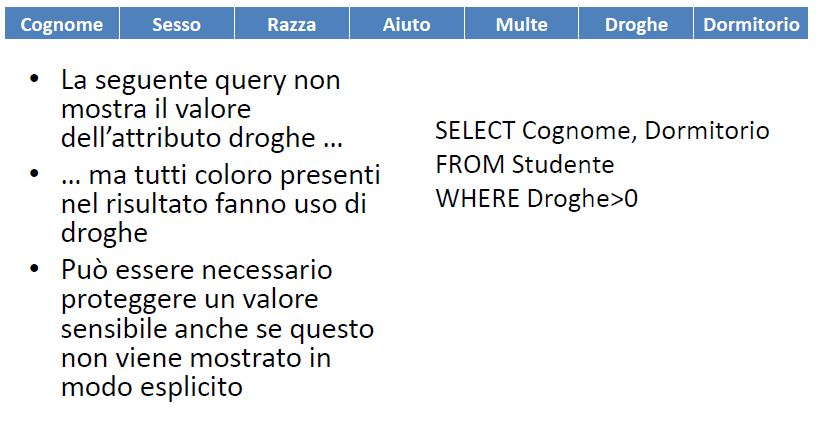
\includegraphics[height=15cm, width=12cm, keepaspectratio]{Immagini/Capitolo10/prot_dati_02.jpg}}
			\caption{Esempio di come ottenere dati sensibili senza leggerli effettivamente \label{fig:query_db}}
\end{figure}

Nella fig. \ref{fig:query_db} si nota come, anche se non si accede fisicamente al campo sensibile, si riesce a dedurlo.
Per poter proteggere i dati si potrebbe pensare di attuare delle politiche sempre più restrittive, ad esempio rifiutare ogni tipo di query che faccia riferimento al campo sensibile...ma ciò va a limitare anche le interrogazioni legittime.
Perciò abbiamo due esigenze contrastanti:
\begin{itemize}

	\item Nascondere i dati per evitare di fornire dati sensibili
	\item Facilitare la divulgazione dei dati non sensibili per consentire l'uso corretto dei dati da parte degli utenti autorizzati
	
\end{itemize}

\begin{figure}[htbp]

	\centering
	{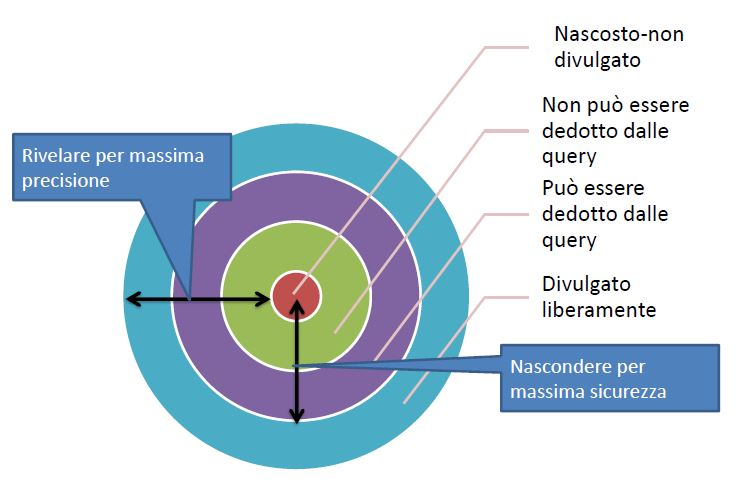
\includegraphics[height=15cm, width=12cm, keepaspectratio]{Immagini/Capitolo10/prot_dati_03.jpg}}
				\caption{Rappresentazione grafica di accessibilità vs. protezione dei dati \label{fig:protezione_vs_accessibilita}}

\end{figure}

\subsection{Tipi di Divulgazione}
La divulgazione può essere suddivisa nei seguenti gruppi:

\begin{itemize}

	\item\textbf{Dati Esatti}: consiste nella divulgazione del valore esatto del campo sensibile, può avvenire per richiesta esplicita o vengono restituiti come parte di una query insieme ad altri dati non sensibili o, addirittura, per errore del sistema
	\item \textbf{Limiti}: si rendono noti gli estremi di variabilità di un dato sensibile, con una ricerca dicotomica si potrebbe arrivare a dedurre un valore molto prossimo a quello esatto. In certi casi, comunque, la semplice conoscenza dei limiti rappresenta una violazione alla sicurezza stessa.
	\item \textbf{Risultato Negativo}: si può dedurre un certo valore anche dal fatto che è uguale ad un altro valore con cui si è fatta la query (se il numero di condanne di una persona non è zero, si sa che quest'ultima è stata condannata almeno una volta)
	\item \textbf{Esistenza}: anche la sola conoscenza di esistenza di un attributo è sensibile
	\item \textbf{Valore Probabile}: tramite l'utilizzo di diverse query e interpolando i dati ottenuti si possono ottenere informazioni non precise, ma attendibili, riguardo i valori di alcuni dati sensibili
\end{itemize}

\section{Inferenza}
L'\textbf{Inferenza} è un metodo per dedurre o derivare dati, sia sensibili che non. Ricordando la tabella di fig. \ref{fig:tabella_db}, una query del tipo è un \textbf{Attacco Diretto}.
\begin{figure}[htbp]

	{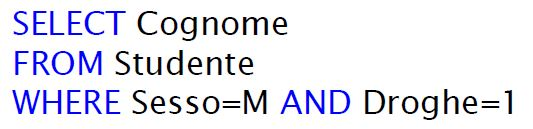
\includegraphics[height=5cm, width=8cm, keepaspectratio]{Immagini/Capitolo10/prot_dati_04.jpg}}
				\caption{Query che sfrutta inferenza per ottenere dati sensibili e viene bloccata \label{fig:query_inferenza}}

\end{figure}

Potrebbe essere rifiutata dal DBMS in quanto le tuple del risultato sono quelle con uno specifico valore su un attributo sensibile.
La seguente query, invece, intuitivamente risulta legale ma va a selezionare solo tuple sensibili, in quanto la seconda e la terza condizione non sono mai soddisfatte.

\begin{figure}[htbp]

	{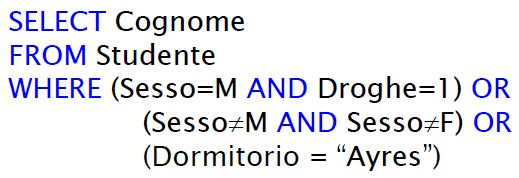
\includegraphics[height=5cm, width=8cm, keepaspectratio]{Immagini/Capitolo10/prot_dati_05.jpg}}
				\caption{Query che sfrutta inferenza per ottenere dati sensibili e non viene bloccata \label{fig:query_inferenza1}}

\end{figure}

Per scovare l'accesso improprio ai dati, il DBMS dovrebbe capire che ci sono solo due valori ammessi per il campo Sesso e che non c'è alcuna tupla con valore Dormitorio uguale ad Ayres.
Per limitare gli Attacchi Diretti è applicata, alle volte, una regola ``\textit{n elementi sul k percento}``, che consiste nel non divulgare se un piccolo numero di elementi divulgati costituisce una grande percentuale del valore restituito dalla query (nel caso precedente un unico elemento era il 100\%).

Un attacco inferenziale \textbf{Indiretto} si basa sulla deduzione di dati sensibile a partire da uno o più dati statistici intermedi.

\subsection{Somma e Conteggio}

Una query del genere \ref{fig:query_indiretta_result} potrebbe sembrare innocua poichè restituisce solo valori aggregati, ma il risultato è una \textbf{Divulgazione di Tipo Negativo}, in quanto posso dedurre dal valore nullo nel dormitorio Holmes che le donne in quel dormitorio nn ricevono aiuti finanziari (che è un dato decretato sensibile). 

\begin{figure}[htbp]
	\centering
	
	\subfigure[Query di attacco indiretto di somma]
		{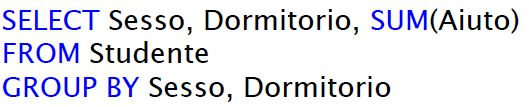
\includegraphics[height=5cm, width=8cm, keepaspectratio]{Immagini/Capitolo10/prot_dati_06.jpg}}
				
	\subfigure[Risultato della query]
		{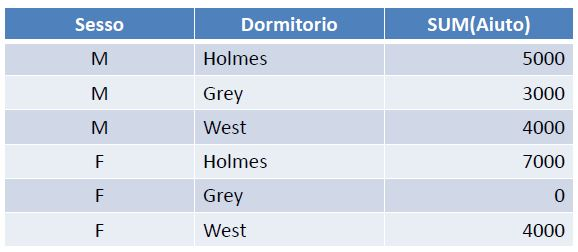
\includegraphics[height=5cm, width=8cm, keepaspectratio]{Immagini/Capitolo10/prot_dati_09.jpg}}
							\caption{Esempio di attacco Indiretto \label{fig:query_indiretta_result}}                           
	
\end{figure}

Inoltre, il conteggio può essere combinato con la somma per produrre risultati ancora più rivelatori!!

\begin{figure}[htpb]
	\centering
	
	\subfigure[Query di attacco indiretto di conteggio]
		{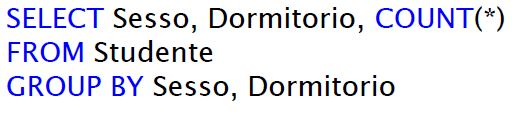
\includegraphics[height=5cm, width=8cm, keepaspectratio]{Immagini/Capitolo10/prot_dati_07.jpg}}
				
	\subfigure[Risultato della query]
		{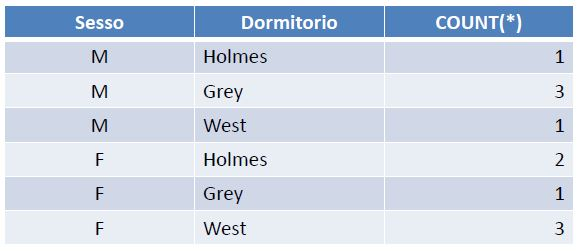
\includegraphics[height=5cm, width=8cm, keepaspectratio]{Immagini/Capitolo10/prot_dati_08.jpg}}
							\caption{Esempio di attacco Indiretto di Somma e Conteggio \label{fig:query_indiretta_result1}}                           
	
\end{figure}

Il risultato della query di \textbf{Attacco di Somma} \ref{fig:query_indiretta_result} combinata con la query di \textbf{Attacco di Conteggio} \ref{fig:query_indiretta_result1} rivela che i due uomini nel dormitorio Holmes e West ricevono un aiuto finanziario di 5000 e 4000.

\subsection{Media}

La media può permettere di ottenere informazioni esatte se utilizzate in combinazione con il conteggio. Usata in modo opportuno riesce anche ad aggirare eventuali controlli sulla numerosità dell'insieme su cui viene calcolata.
Ad esempio, supponiamo che la media non venga divulgata se la somma degli elementi su cui è calcolata è pari ad 1 (legge interna del DBMS). 

\begin{figure}[htpb]
	\centering
		\subfigure[Query di Media per ottenere informazioni sugli studenti di Sesso Femminile]
		{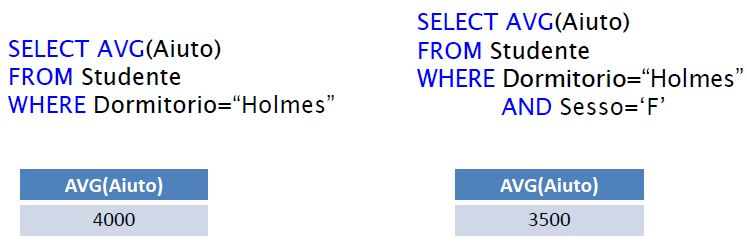
\includegraphics[height=2cm, width=8cm, keepaspectratio]{Immagini/Capitolo10/prot_dati_10.jpg}}
		
		\subfigure[Query di Count da combinare con la Query di Media per ottenere un Attacco Inferenziale]
		{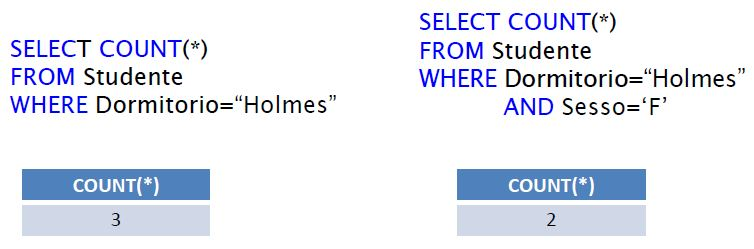
\includegraphics[height=2cm, width=8cm, keepaspectratio]{Immagini/Capitolo10/prot_dati_11.jpg}}
		
		\subfigure[Combinazione delle informazioni ottenute]
				{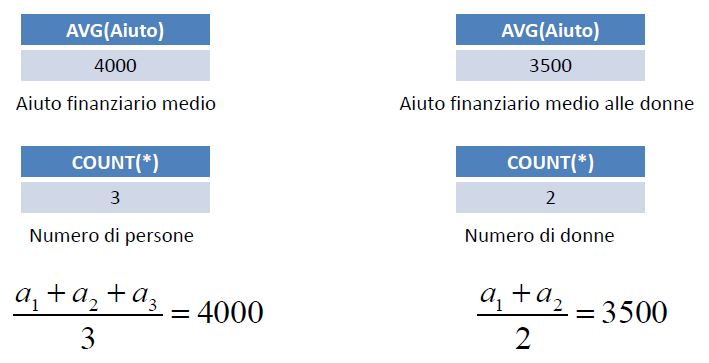
\includegraphics[height=2cm, width=8cm, keepaspectratio]{Immagini/Capitolo10/prot_dati_12.jpg}}
		
		\caption{Esempio di query di media per ottenere indirettamente informazioni 
		  \label{fig:query_media}}  

\end{figure}

Dalla procedure di \ref{fig:query_media} si trova che $ a_{3} = 5000 $ che sarebbe un dato sensibile, in quanto media di un valore su un unico elemento!

\subsection{Attacchi di Tracker}
Abbiamo visto che una delle tecniche di protezione dall'inferenza consiste nel non divulgare i dati se solo un piccolo numero di elementi fornisce molta informazione; è possibile aggirare questa limitazione effettuando più query lecite e combinandole insieme. 

\begin{figure}[htpb]
\centering
	{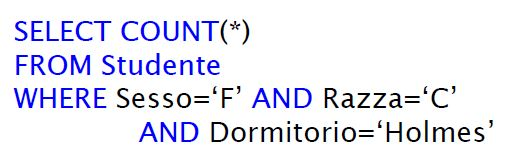
\includegraphics[height=5cm, width=8cm, keepaspectratio]{Immagini/Capitolo10/prot_dati_13.jpg}}
		\caption{Esempio di query di tracker non lecita du DB
				  \label{fig:query_tracker_sbagliata}}  
\end{figure}

La query \ref{fig:query_tracker_sbagliata} è, ovviamente, bloccata dal DBMS in quanto va a richiedere un unico risultato sulla tabella del DB in fig. \ref{fig:tabella_db}.
Il dato non viene divulgato in quanto \underline{dominato da una sola tupla}, ma osserviamo che il dato in questione pò essere calcolato contando partendo dal fatto che tutte le donne non sono di razza \textit{C} o che non risiedono nel dormitorio Holmes.

\begin{figure}[htpb]
\centering
	{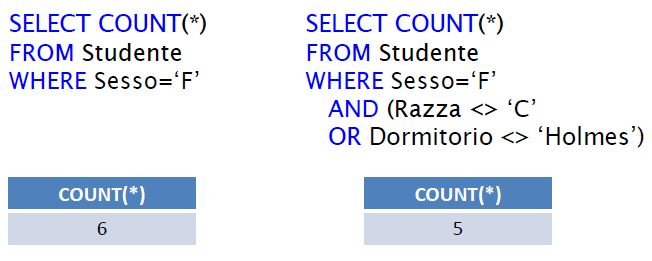
\includegraphics[height=5cm, width=8cm, keepaspectratio]{Immagini/Capitolo10/prot_dati_14.jpg}}
		\caption{Esempio di query di tracker non lecita du DB
				  \label{fig:query_tracker}}  
\end{figure}

\subsection{Vulnerabilità del Sistema Lineare}
L'attacco di Tracker è un caso specifico di una vulnerabilità più generica in cui sfruttando l'algebra, la logica e un pò di fortuna si riesce ad ottenere tramite diverse query dei valori protetti.
\newpage
Nell'esempio \ref{fig:query_tracker} la query protetta è del tipo \textit{q = COUNT\{(Sesso = F)}$\wedge$\textit{(Razza = C)}$\wedge$\textit{(Dormitorio = Holmes)\}}.
\newline
In base all'algebra, possiamo riscrivere la query nel seguente modo: 
\textit{q = COUNT(Sesso = F)}$-$\textit{COUNT\{(Sesso = F)}$\neg$\textit{(Razza = C)}$\wedge$\textit{(Dormitorio = Holmes)\}}.
\newline
Più in generale potremmo avere le seguenti query:
\newline
$q_{1} = c_{1} + c_{2} + c_{3} + c_{42}$
\newline
$q_{2} = c_{3} + c_{2} $
\newline
$q_{3} = c_{5} + c_{1} + c_{3}$
\newline
$q_{4} = c_{4} + c_{7} + c_{2}$
\newline
$q_{5} = c_{8} + c_{3}$
Nessuna delle query rivela un qualsiasi valore $c_{i}$ ma, risolvendo il sistema, possiamo conoscerli tutti.

\subsection{Aggregazione}
L'aggregazione è un altro particolare tipo di inferenza, in cui si cerca di ottenere dati sensibili mettendo insieme dati non sensibili (ad esempio il nome di un impiegato e il suo stipendio, divisi non sono dati sensibili ma insieme si). 
\newline
Evitare l'aggregazione è difficile perché bisogna tenere conto delle informazioni giù in possesso dell'utente. Se un utente conosce il nome di un dipendente non devo comunicargli lo stipendio e viceversa. Purtroppo tenere traccia di tutti i dati rivelati ad ogni utente è proibitivo, soprattutto per il fatto che utenti diversi potrebbero condividere tutti le informazioni in loro possesso.
\newpage
\section{Protezione dall'Inferenza}
Esistono alcune tecniche per combattere l'inferenza: 
\begin{itemize}
\item Analisi delle query
\item Soppressione dei valori sensibili per non fornirli
\item Occultamento del valore reale, con un altro simile
\end{itemize}

\subsection{Soppressione e Occultamento}
Un esempio di soppressione è la già citata regola del ``\textit{n elementi sul k percento}``; purtroppo, per essere efficace, può essere necessario sopprimere altri dati per evitare che quelli sensibili siano ottenibili per differenza.

\begin{figure}[htpb]
	\centering
		\subfigure[Numero di residenti per Sesso e Dormitorio]
		{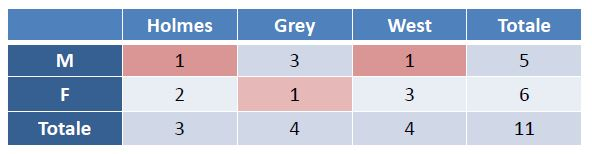
\includegraphics[height=2cm, width=8cm, keepaspectratio]{Immagini/Capitolo10/prot_dati_15.jpg}}
		
		\subfigure[Tabella dopo la soppressione]
		{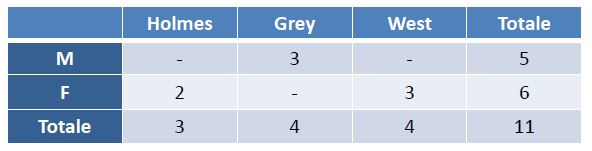
\includegraphics[height=2cm, width=8cm, keepaspectratio]{Immagini/Capitolo10/prot_dati_16.jpg}}
				
		\caption{Esempio di protezione per soppressione
		  \label{fig:query_soppressione}}  

\end{figure}
Per evitare di divulgare dati sensibili è possibile combinare più righe o colonne, implementando una protezione dei dati di Occultamento.

\begin{figure}[htpb]
	\centering
		\subfigure[Numero di residenti per Sesso e Uso di Droghe]
		{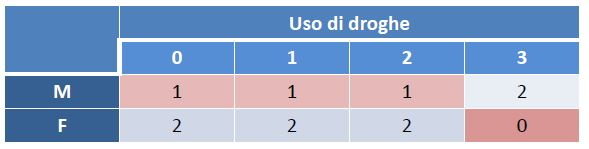
\includegraphics[height=2cm, width=8cm, keepaspectratio]{Immagini/Capitolo10/prot_dati_17.jpg}}
		
		\subfigure[Tabella dopo l'occultamento]
		{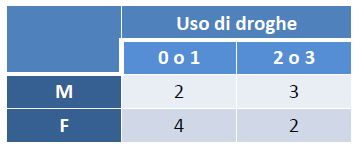
\includegraphics[height=2cm, width=8cm, keepaspectratio]{Immagini/Capitolo10/prot_dati_18.jpg}}
				
		\caption{Esempio di protezione per occultamento
		  \label{fig:query_occultamento}}  

\end{figure}


Nel caso \ref{fig:query_occultamento} la query viene eseguita su di un \textbf{Campione Casuale} dei dati, il campione deve essere abbastanza ampio da rappresentare l'intera popolazione. In questo modo i dati sono sempre rappresentativi ma si diminuisce la possibilità di attacchi statistici.

\subsection{Perturbazione Casuale dei dati}
A volte può essere utile perturbare i valori del DB con un piccolo errore, per ogni $x_{i}$ che rappresenta il valore vero dell'attributo i si può generare un piccolo errore $e_{i}$ e aggiungerlo a $x_{i}$ per calcolare dati statistici.
Valori di query aggregate, quali la somma o la media, produrranno valori vicini a quelli veri ma non esatti.
